\section{Ejercicio 2}

En este ejercicio se busca calcular la activación, función de costo y todos los gradientes involucrados en una red neuronal para la arquitectura de un perceptrón compuesto por dos neuronas + bias con funciones de activación \textbf{sigmoide} y la función de costo es \textbf{MSE}.
La entrada a la red neuronal es $\vec{x}=[-3.1, 1.5]$, $W=[[-0.2, 2],[-0.5, -0.3]]$, $b_1=-4$ y $b_2=-1$.

La función de costo MSE se calcula como:
% \begin{equation}
\begin{align}
    MSE&=\frac{1}{n}\sum^n_{i=1}(\hat{Y_i}-Y_i)^2,\\
    MSE'&=\frac{1}{n} 2 \sum (\hat{Y_i}-Y_i),
\end{align}
donde $n$ es el número de entradas, en este caso 2, $\hat{Y_i}$ es el vector estimado y $Y_i$ es el vector de resultados esperado.
% \end{equation}

El grafo de este problema puede graficarse como:

% \vspace{1cm}
% \hspace{1.5cm}
\begin{figure}[H]
    \centering
    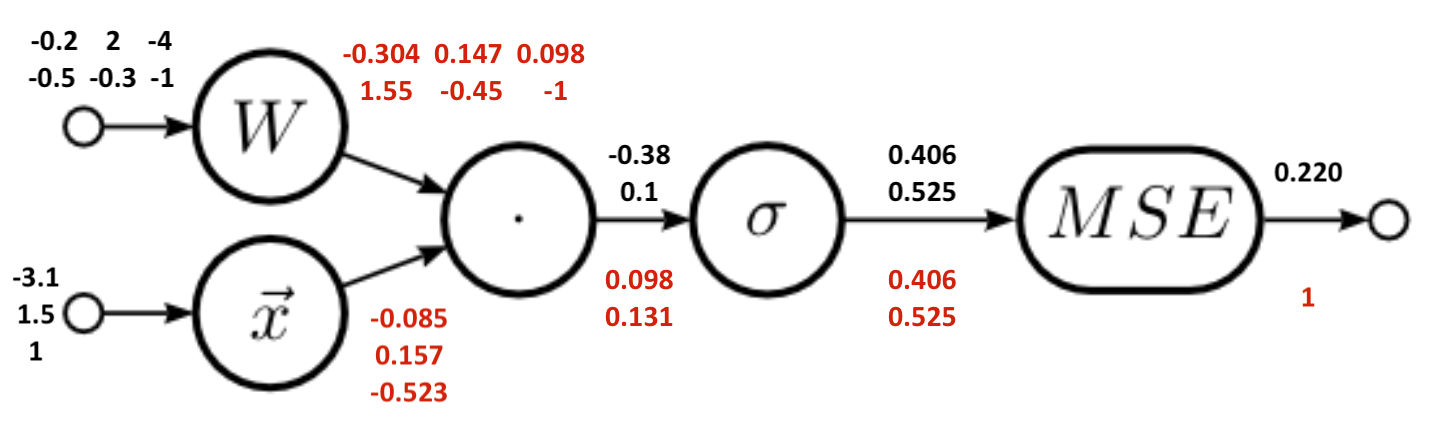
\includegraphics[height=1in]{image/ej2.png}
    \caption{Grafo del ejercicio 2}
    \label{fig:my_label}
\end{figure}
donde nuevamente los valores en negro representan la evaluación hacia adelante de la red y los valores en rojo son los valores calculados durante el \textbf{backpropagation}.

